\documentclass{article}
\usepackage{graphicx}
\usepackage{amsmath}
\usepackage{pgfplots}
\usepackage[margin=1.5cm]{geometry}
\usepackage{adjustbox}
\usepackage{hyperref}
\usepackage{cite}
\usepackage{listings}
\usepackage{xcolor}
\usepackage{comment}
\usepackage{graphicx}
\usepackage{pdfpages}
\usepackage{enumitem}
\usepackage[utf8]{inputenc}
\lstset{ 
literate= {á}{{\'a}}1 
    {é}{{\'e}}1 
    {í}{{\'i}}1 
    {ó}{{\'o}}1 
    {ú}{{\'u}}1
} 

\hypersetup{
colorlinks=true,
linkcolor=blue,
urlcolor=blue,
}

\pgfplotsset{compat=1.17}
\usepackage[portuguese]{babel}

\definecolor{codegreen}{rgb}{0,0.6,0}
\definecolor{codegray}{rgb}{0.5,0.5,0.5}
\definecolor{codepurple}{rgb}{0.58,0,0.82}
\definecolor{backcolour}{rgb}{0.95,0.95,0.92}

\lstdefinestyle{mystyle}{
    backgroundcolor=\color{backcolour},   
    commentstyle=\color{codegreen},
    keywordstyle=\color{magenta},
    numberstyle=\tiny\color{codegray},
    stringstyle=\color{codepurple},
    basicstyle=\ttfamily\footnotesize,
    breakatwhitespace=false,         
    breaklines=true,                 
    captionpos=b,                    
    keepspaces=true,                 
    numbers=left,                    
    numbersep=5pt,                  
    showspaces=false,                
    showstringspaces=false,
    showtabs=false,                  
    tabsize=2
}

\lstset{style=mystyle}

\title{Lista Árvore}
\author{Gabriel de Paula Gaspar Pinto}
\date{}

\begin{document}

\maketitle

\section{Introdução}
\paragraph{}Nesse trabalho, foi realizada os exercícios da "Lista árvore", disponível no Classroom, da matéria de Estrutura de Dados. Para realizar esta lista, foi utilizado o aplicativo Samsung Notes, em um tablet Android, para facilitar a visualização das árvores feitas manualmente e não precisar usar papel. Para confecção dos códigos, foi utilizado o Visual Studio Code, dentro do ambiente virtual do Windows Subsystem for Linux (WSL), além de auxílio da inteligência artifical generativa, ChatGPT.

\section*{Lista de Exercícios}

\textbf{Questão 1:}

\begin{enumerate}[label=(\alph*)]
    \item A árvore com meu nome completo, tem altura 8, considerando que a raiz está no nível 1.
    \item Em um percurso pós-fixado(pós-ordem), a ordem dos nós fica da seguinte maneira:
    A A A D E A E B A O N P L P I P G L I R T S U R G.
    \item O sucessor do nó de maior altura é a letra A.
    \item O quarto nó inserido na árvore, é a letra R (G A B \textbf{R} I E L), então o seu predecessor é o nó raiz da árvore, com a letra G.
    \item Na figura 2 está o resultado da árvore quando se remove o nó raiz (G), resultado do maior nó dentro da subárvore da esquerda.
\end{enumerate}

Abaixo estão as imagens da árvore binária de busca completa e a árvore com a raiz removida.

\begin{figure}[h!]
    \centering
    % Primeira imagem
    \begin{minipage}{0.45\linewidth}
        \centering
        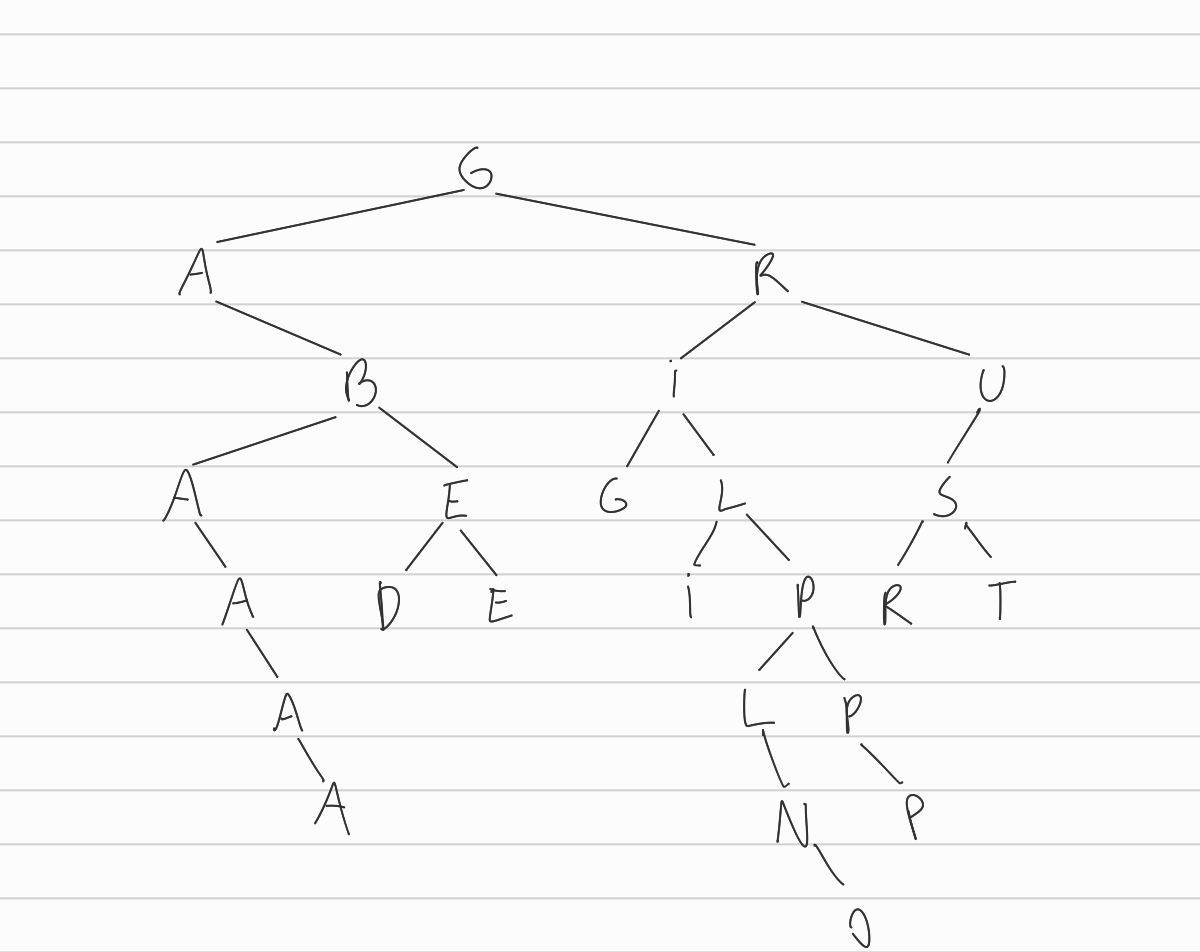
\includegraphics[width=\linewidth]{arvoredebusca.jpg}
        \caption{Árvore Binária de Busca completa}
        \label{fig:arvorecompleta}
    \end{minipage}
    \hfill
    % Segunda imagem
    \begin{minipage}{0.45\linewidth}
        \centering
        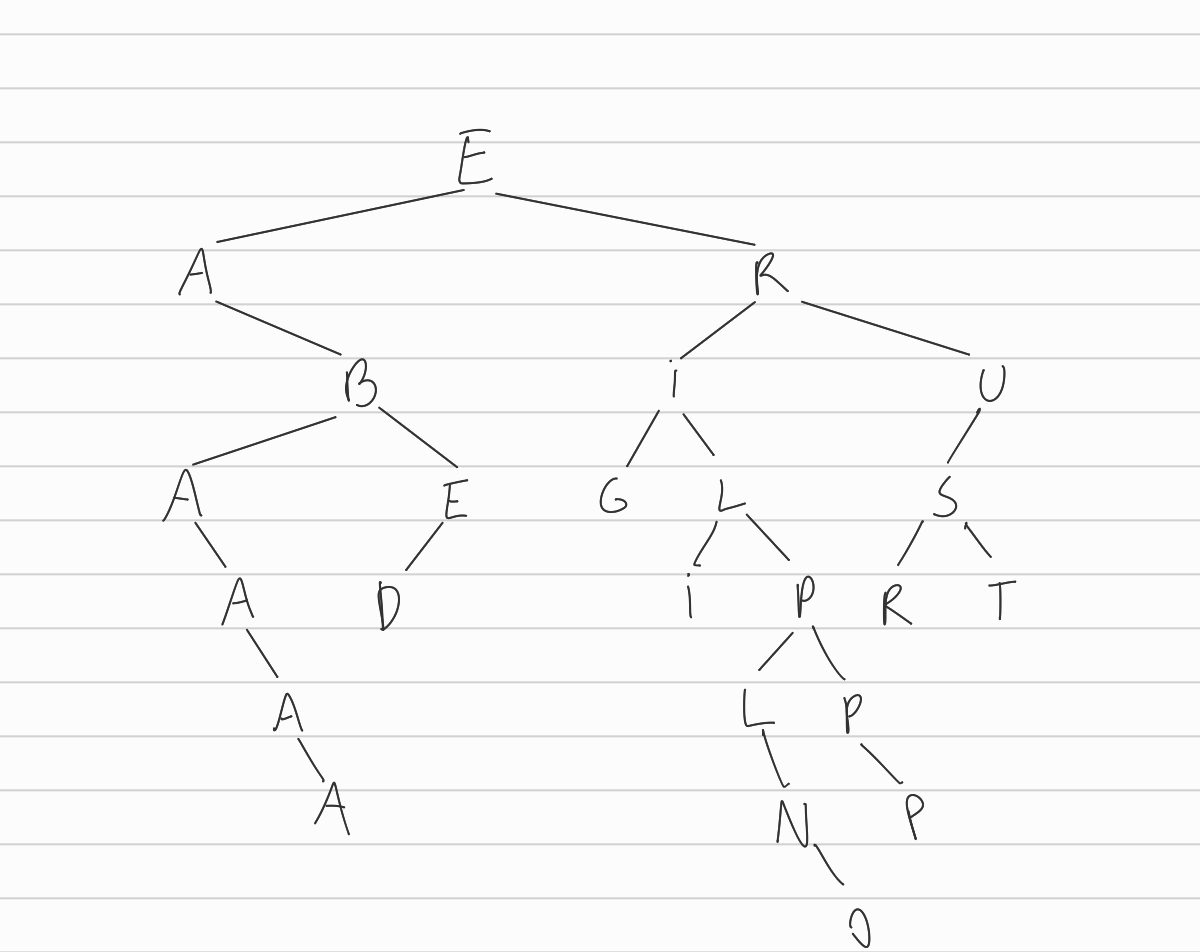
\includegraphics[width=\linewidth]{raizremovida.jpg}
        \caption{Árvore Binária de Busca após remover a raiz}
        \label{fig:arvoresemraiz}
    \end{minipage}
\end{figure}

\newpage
\textbf{Questão 2:}
Ao montar a árvore de Huffmann, com meu nome completo e sem espaços, fica do jeito que mostra na imagem a seguir

\begin{figure}[h!]
    \centering
    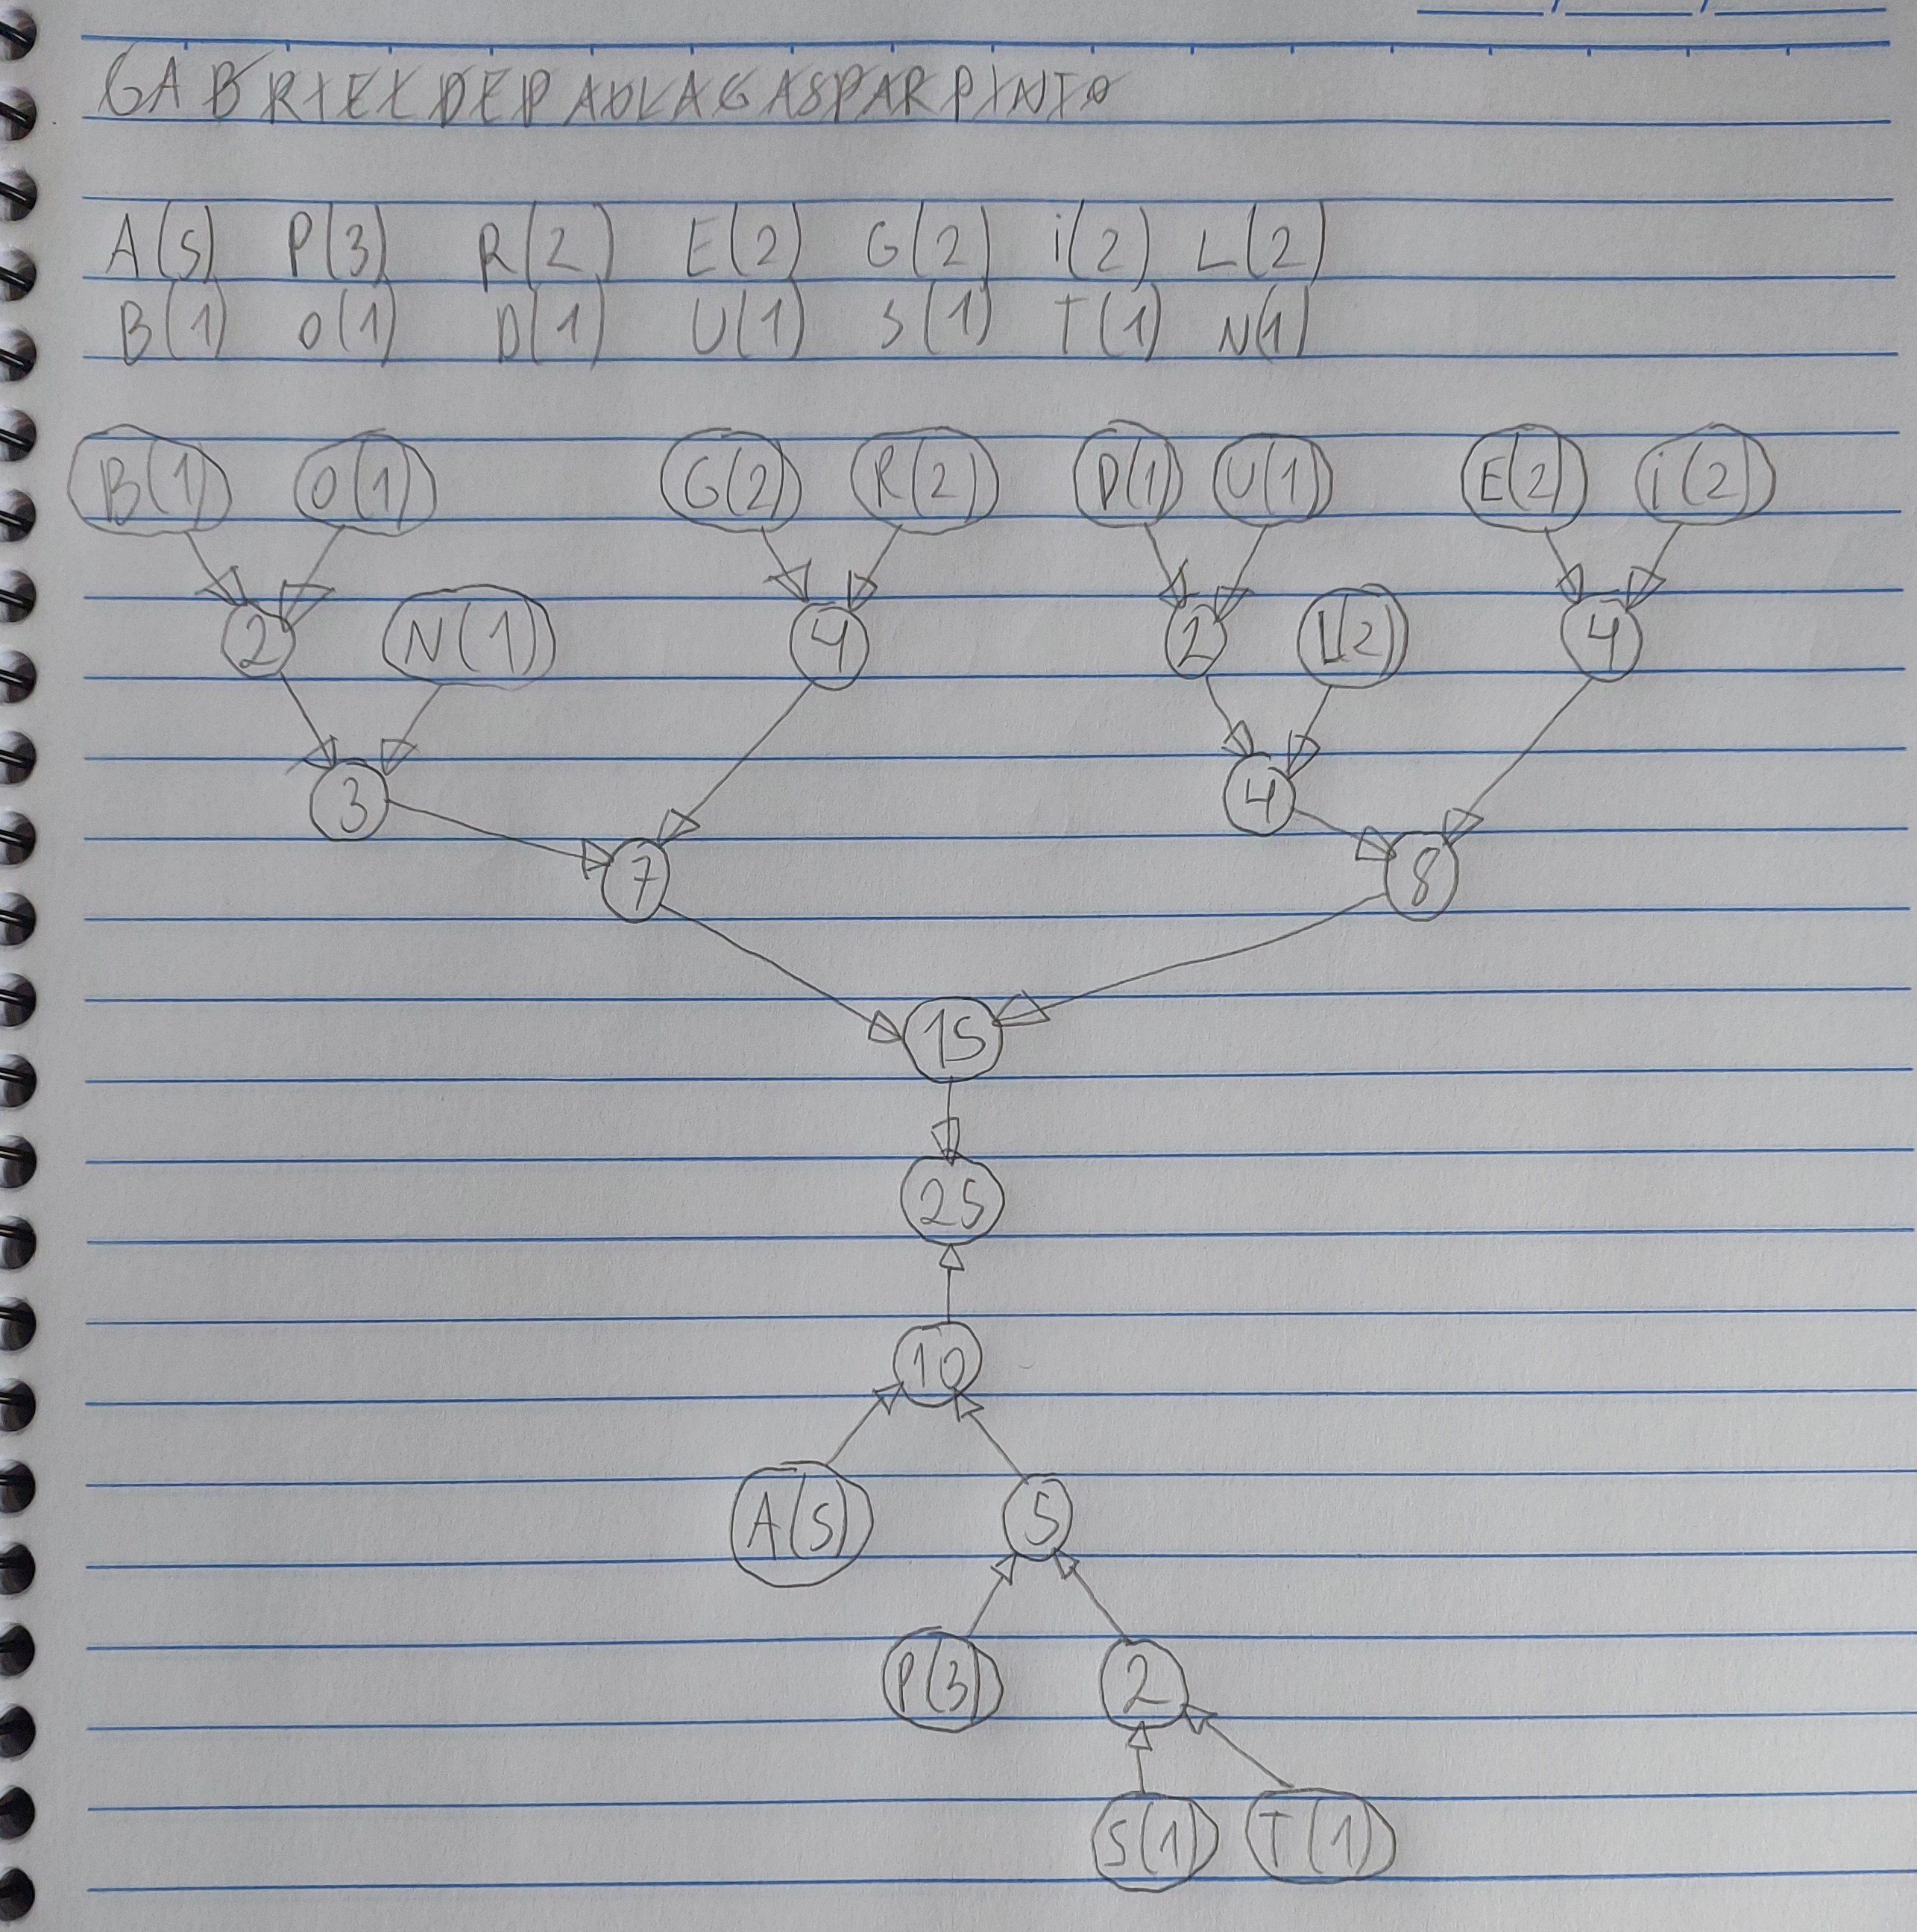
\includegraphics[width=0.5\linewidth]{huffmann.jpg}
    \caption{Árvore de Huffmann, com meu nome completo}
    \label{fig:questao1}
\end{figure}

\textbf{Questão 3:}
A seguir está o meu código para calcular a altura de uma árvore binária de pesquisa. Para poder testar o código, eu inseri a árvore binária de pesquisa do meu nome, presente na questão 1. Neste caso, quando rodar o programa, o resultado impresso na tela é 8.

\lstinputlisting[language=c++]{code/alturaArvore.cpp}

\newpage
\textbf{Questão 4:}
A seguir está o meu código para calcular o nível (altura) de um nó em uma árvore. Para poder testar o código, eu também inseri a árvore binária de pesquisa do meu nome, presente na questão 1. Os resultados são das letras A, L, P, U, O e da raiz (letra G), respectivamente. Neste caso, os resultados que o programa deve mostrar são, respectivamente: 2, 4, 5, 3, 8 e 1. Para alterar os valores procurados, é necessário somente mudar o valor do meio quando as funções são chamadas, dentro do cout, considerando que cada letra equivale a um número, sendo A = 1, B = 2 e assim por diante.

\lstinputlisting[language=c++]{code/alturaNo.cpp}

\section{Nota}
\paragraph{}Como este arquivo \LaTeX  \hspace{1mm}utiliza arquivos externos (para imagens e códigos-fonte), este trabalho está disponivel em um repositório pessoal do GitHub, junto com todos os outros trabalhos que eu utilizei \LaTeX.

\begin{center}
    \href{https://github.com/gpgp2006/LaTeX}{GitHub - \LaTeX}

    
\end{center}

\end{document}